In this section, we evaluate the performance of the proposed framework. The
source code of all the parts of the experimental setup along with all the pieces
of input data mentioned in this section are available online \cite{sources}. In
particular, \cite{sources} contains a system simulator needed for the quantities
introduced in \sref{modeling} and an implementation of the interpolation
algorithm introduced in \sref{interpolation}. For the most part, the utilized
programming language is Go. The experiments are conducted on a GNU/Linux machine
equipped with 16 processors Intel Xeon E5520 2.27~GHz and 24~GB of RAM.

Heterogeneous platforms and applications used in our experiments are generated
by the \abbr{TGFF} tool \cite{dick1998}. For each considered problem, the tool
generates (i) a directed acyclic graph representing a set of tasks along with
their data dependencies and (ii) a number of tables representing a set of
processing elements. Each table assigns two numbers to each task: a best-case
execution time and a power consumption. The two numbers characterize the task if
it is executed on the processing element that the table corresponds to. The
best-case execution time is chosen uniformly between 1 and 50~ms, and it is used
for assigning a probability distribution to the execution time of the task,
which will be discussed shortly. The power consumption is chosen uniformly
between 10 and 50~W, and it is assumed to remain fixed thereafter. The
floorplans of the platforms are constructed to form regular grids wherein each
processing element occupies $4 \times 4~\text{mm}^2$ on the die. The
applications are scheduled using a static cyclic scheduler following the list
scheduling policy \cite{adam1974}. The mapping of the tasks onto the processing
elements is assumed to be fixed.

\begin{figure}[t]
  \centering
  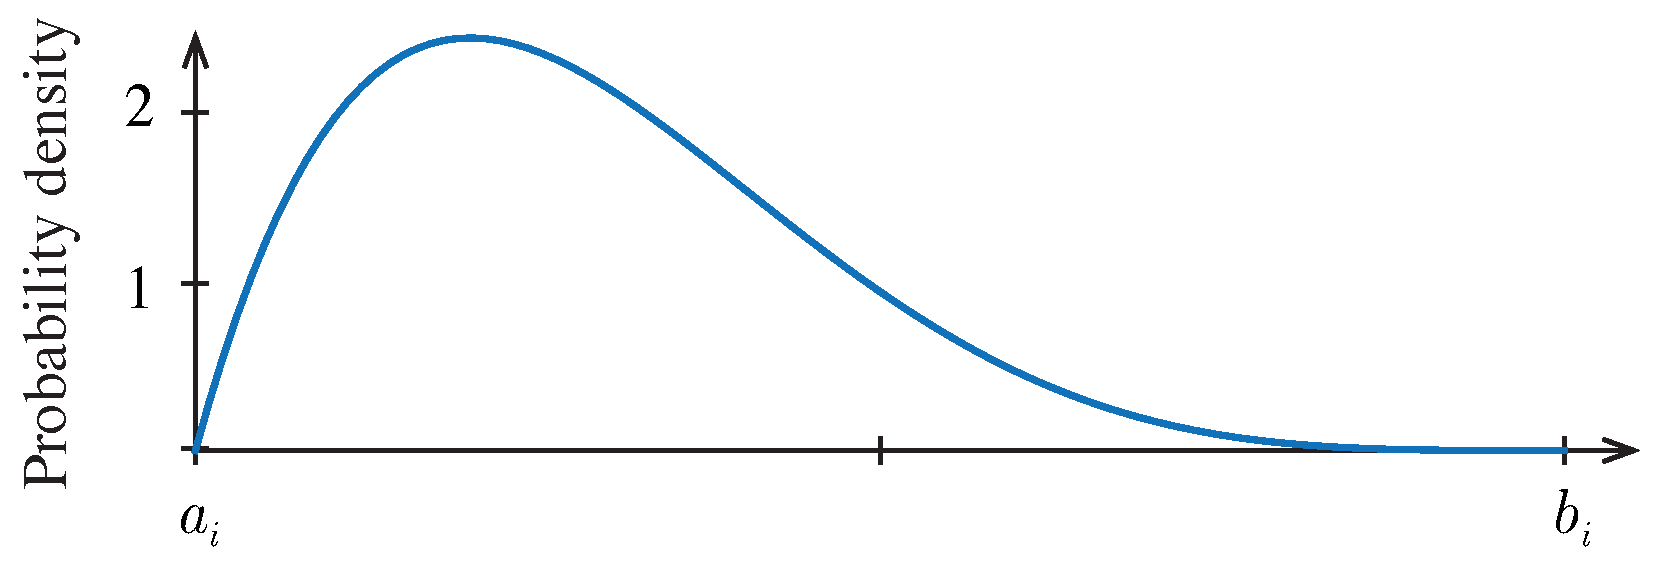
\includegraphics[width=1.0\columnwidth]{include/assets/figures/beta.pdf}
  \caption{The probability density of the beta distribution $\text{Beta}(2, 5, a_i, b_i)$.}
  \flab{beta}
\end{figure}

For illustration purposes, the uncertain parameters are assumed to be the
execution times of the tasks; in other words, $\vu = \vb$ and $\nu = \nt$.
Without loss of generality, the distribution of $\u_i$ or, equivalently, $\b_i$
is assumed to be a four-parametric beta distribution $\text{Beta}(\alpha_i,
\beta_i, a_i, b_i)$ where $\alpha_i$ and $\beta_i$ are the shape parameters, and
$a_i$ and $b_i$ are the endpoints of the support. The parameters $\alpha_i$ and
$\beta_i$ are set to 2 and 5, respectively, for all tasks. The left endpoint
$a_i$ is set to the best-case execution time of the task generated by the
\abbr{TGFF} tool, and the right endpoint $b_i$ is set to be 20\% larger than
$a_i$. The shape of such distributions is illustrated in \fref{beta}. The
correlations between the tasks of an application are generated based on the
structure of the corresponding directed acyclic graph produced by the
\abbr{TGFF} tool: the closer two tasks are in the graph, the stronger the
correlation between their execution times.

The construction of thermal \abbr{RC} circuits for the considered multiprocessor
platforms is delegated to the HotSpot tool \cite{skadron2004}; the output of the
tool is essentially a pair of a thermal capacitance matrix $\mC$ and a thermal
conductance $\mG$ matrix that appear in \eref{thermal-system}. The granularity
of power and temperature profiles, discussed in \sref{power-consumption} and
\sref{heat-dissipation}, is set to $10^{-5}$~s; in practice, this sampling rate
should be set to a value that is reasonable for the problem at hand.

Regarding interpolation, we rely on the open Newton--Cotes rule, as motivated in
\sref{collocation-nodes}. The \token{IsLimitReached} subroutine in
\aref{construct} terminates the algorithm when it reaches a certain
interpolation level. The decision taken in \token{IsAccurateEnough} is based on
\eref{absolute-error} and \eref{relative-error}.

Lastly, let us remind that our experimental setup is publicly available
\cite{sources}. The configuration aspects that have not been explicitly
mentioned here can be found online, and the results presented below can be
readily reproduced.

\subsection{Application Timing}
The quantity of interest $\g$ considered in this subsection is the end-to-end
delay given in \eref{end-to-end-delay}, which is a scalar.

\subsection{Power Consumption}
Let the quantity of interest $\g$ be the total energy given in
\eref{total-energy}, which is a scalar.

\subsection{Heat Dissipation}
In this subsection, the quantity of interest $\g$ is the temperature profile
$\mQ$ of the system calculated using \eref{thermal-system}. The profile is an
$\np \times \ns$ matrix, and, therefore, $\g$ is $\np \ns$-dimensional.
